\begin{tikzpicture}[align=center, arrow/.style={very thick, line cap=round, -{Latex[length=2.5mm]}}, font=\footnotesize]
    \matrix[inner sep=0pt, column sep=4em, row sep=0pt] (mtx1) {
        \node[inner sep=0pt] (step0) {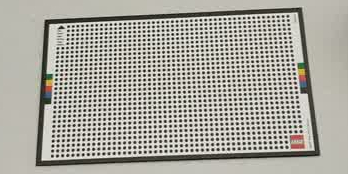
\includegraphics[height=.2\textheight]{img/lego/img0.jpeg}};
        & \node[inner sep=0pt] (step1) {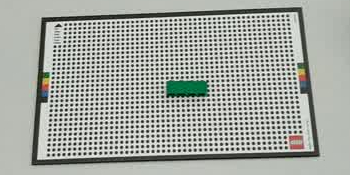
\includegraphics[height=.2\textheight]{img/lego/img1.jpeg}};\\
    };

    \node[inner sep=2mm, text width=11em, draw, rectangle, very thick, below=3em of mtx1] 
    (instruction) {Example instruction:\\``Put the white 1x1 brick on top of the green 1x4 brick.''};

    \matrix[inner sep=0pt, column sep=4em, row sep=0pt, below=3em of instruction] (mtx2) {
        \node[inner sep=0pt] (step2) {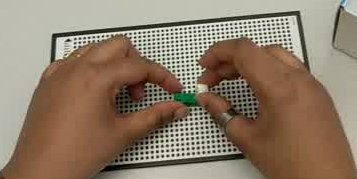
\includegraphics[height=.2\textheight]{img/lego/img2.jpeg}};
        & \node[inner sep=0pt] (step3) {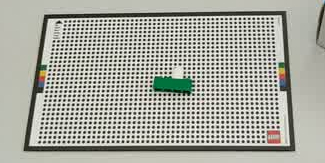
\includegraphics[height=.2\textheight]{img/lego/img3.jpeg}};\\
    };

    \coordinate[right=2em of step1.east] (a1);
    \coordinate[left=2em of step2.west] (a2);

    \begin{scope}[arrow]
        \draw (step0) -- node[midway, above, sloped] {\Large\ldots} (step1);
        \draw (step2) -- node[midway, above, sloped] {\Large\ldots} (step3);
        \draw (a1) |- (instruction);
        \draw (a2) -- (step2);
    \end{scope}

    \begin{scope}[very thick, line cap=round]
        \draw (step1) -- (a1);
        \draw (instruction) -| (a2);
    \end{scope}

    \node[fit=(step0) (step1), draw, rectangle] (fit1) {};
    \node[fit=(step2) (step3), draw, rectangle] (fit2) {};

    \node[inner sep=0mm, below=1mm of fit1.south] (label1) {Step $N$};
    \node[inner sep=0mm, above=1mm of fit2.north] (label2) {Step $N+1$};

\end{tikzpicture}